\chapter{多用户下的可验证对称加密搜索方案研究}
\label{cha:multi-user}
\section{引言}

\section{系统架构}

\begin{figure}[t]
\centering
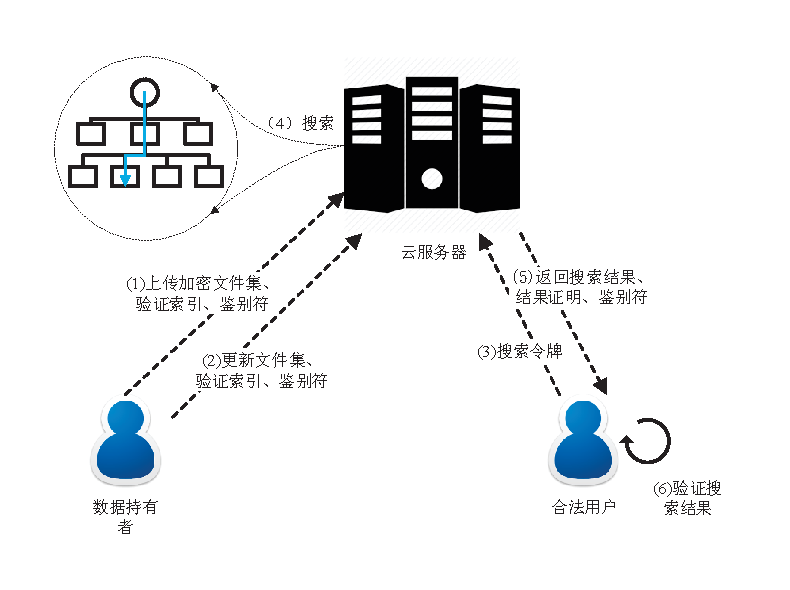
\includegraphics[width=6 in]{fig/GM-VSSE}
\DeclareGraphicsExtensions.
\caption{多用户场景下的可验证对称加密搜索框架\multi}
\label{fig:GM-VSSE}
\end{figure}


\section{方案流程} 三方

\section{算法分析}
\subsection{构建时间戳链}

In order to prevent cloud services from replaying previous authenticators and ensure the freshness of the root, we maintain a timestamp-chain for authenticators, such that users can trace authenticators in the chain and identify if the root is fresh. %, which is important to ensure the correctness of search verification.
Here, the timestamp-chain scheme is different from the timestamp mechanism used in SSE~\cite{stefanov2014practical}. Their schemes can only prevent servers from constructing data freshness attacks under the two-party model when the user holds the update information. Unfortunately, it may not be able to detect data freshness attack in our concerned three-party model. We show the details of our scheme below.
Firstly, we will show how the data owner creates the authenticator by leveraging the timestamp-chain. In the very beginning, a data owner sets an interval for authenticator update\footnote{In the performance evaluation section, i.e., Section~\ref{sec:experiments}, we will show the relationship between the update interval and the delays of detecting data freshness attacks.}, and then the fixed update time points are set to be $\{up_1, up_2, \cdots, up_i, \cdots, up_m\}$ (see Fig.~\ref{fig:timestamp}).
Here, we use Network Time Protocol (NTP)~\cite{mills1991internet, mills2010network} run on cloud servers
to synchronize the clocks among the data owners and the data users
during their interactions with the servers. The clock synchronization
accuracy can reach a few milliseconds or even tens of microseconds~\cite{kopetz1987clock, elson2002fine, zhou2007accurate}, and thus the accuracy is enough for verification in
GSSE. Note that, a malicious server can possibly fake a clock,
%However, it cannot fake the timestamp chain, since its goal is to allow users to successfully verify search results. a fake timestamp will olead to a fail result.
%A malicious server can indeed fake clocks,
but it cannot fake the timestamp-chain. If the server faked the clock, the timestamp will not allow a server to bypass the verification performed by users.
The authenticator is uploaded to the server periodically at the update time point when there is no data update in an update interval. Otherwise, the data owner will additionally upload the authenticators along with the updating data.


Intuitively, in order to prevent the authenticator from being replayed, we can simply set the authenticator $\pi$ as a concatenation of timestamp $tp$ and the root of the MPT, i.e., the proof index, encrypt it by using a symmetric key $K_3$, and then sign it with the secret key $ssk$. If the proof index is not updated during an update interval, the data owner only needs to update the timestamp at next update time point. If the document set of the data owner is modified within an update interval, which means the root of the proof index has been updated, then the data owner will calculate a new authenticator by using the latest root and the current timestamp and upload it to cloud services again. %{\bf In this setting, the server cannot infer relationship between authenticators during two different update intervals.??}
In this setting, when a data user generates a challenge, the server should send the latest authenticator to the data user. The data user can recover the root and the timestamp by decrypting the authenticator. If the timestamp is beyond the valid time, i.e., before the latest update time point, then the server is considered as malicious. This mechanism ensures that the server cannot mount a data freshness attack by using the data before the latest update time point.

However, cloud services may still be able to replay the authenticator between the latest update time point and the current query time. Specifically, if there is one or more data updates happened after the latest update time point, then the server can cheat the data user by sending any authenticator uploaded after the latest update time point and then mounts a data freshness attack within the latest update interval.
Therefore, we develop a timestamp-chain mechanism to detect those cheating behaviors. We modify the structure of the authenticator by chaining the value of the previous authenticator into the newly generated authenticator according to Equation (1). Note that, it will generate a new timestamp-chain of a new update interval, while the timestamp-chain ends at the beginning of the next update interval. In other words, the authenticators in each update interval are chained together, e.g., $\pi_{i, 0}, \pi_{i, 1}$ (see Fig.~\ref{fig:timestamp}), but the authenticators are irrelevant in the two different update intervals. Here, the last authenticator in each update interval is uploaded at the next update time point. In this setting, the server needs to provide an authenticator at the query time and meanwhile an authenticator at the checkpoint, where the checkpoint is referred as the next update time point closest to the user's query time $t$, e.g., $up_{i+1}$ is the checkpoint in the update interval $(up_i,up_{i+1}]$.

\begin{equation}
    \left\{
    \begin{array}{ll} % \begin{eqnarray}好像也可以。
      \pi_{i, 0} = (\alpha_{i, 0}, \mathsf{Sig}_{ssk}(\alpha_{i, 0})),~~~~~~~~~~~up_i < tp_{i, 0} \leq up_{i+1} \\
      \alpha_{i, 0} = Enc_{K_3}(rt_{i, 0}||tp_{i, 0}) \\
      \cdots \\

     \pi_{i, j} = (\alpha_{i, j}, \mathsf{Sig}_{ssk}(\alpha_{i, j})),~~~~~~~~~~~tp_{i, j-1} < tp_{i, j} \leq up_{i+1}  \\
     \alpha_{i, j} = Enc_{K_3}(rt_{i, j}||tp_{i, j}||\alpha_{i, j-1}) \\
      \cdots  \\
     \pi_{i, n} = (\alpha_{i, n}, \mathsf{Sig}_{ssk}(\alpha_{i, n})),~~~~~~~~~~~tp_{i, n}=up_{i+1} \\
     \alpha_{i, n} = Enc_{K_3}(rt_{i, n}||tp_{i, n}||\alpha_{i, n-1})
    \end{array}
    \right.
  \end{equation}

\noindent Here $i$ represents the $i$-th update interval and $j$ represents the $j$-th authenticator in the interval.

Let us consider the following cases (shown in Fig.~\ref{fig:timestamp}) when a data user initiates a query at different time points: (i) the first case is that the query occurs at $t_1$, where $t_1 < tp_{i, 0}$, the server can only send $\pi_{i-1, n}$ to the data user; (ii) the second case is that the query occurs at $t_2$ after the data update event at $tp_{i, 0}$, and the authenticator that server sends to the user is $\pi_{i, 0}$; (iii) the last case is that the query is generated at $t_2$, and the authenticator sent by the server is $\pi_{i-1, n}$. In the last case, a data freshness attack occurs, but it will be detected at the checkpoint $up_{i+1}$. The data user will obtain the last authenticator $\pi_{i, 1}$ from the server at the checkpoint to verify whether the data obtained at the query time has been replayed or not.

\subsection{验证时间戳}
Algorithm~\ref{alg:check} shows the pseudo-code of the {\it Check} algorithm that is executed by a data user and verifies whether the authenticator has been replayed. Let $\pi^t_q$ denote the authenticator received at the query time $t$ and $\pi_c$ denote the authenticator received at the checkpoint, which is used to deduce the previous authenticators during the latest update interval. First, we need to verify the signature of $\pi^t_q$ and $\pi_c$ by using the public key $spk$ of the data owner. We check the authenticator $\pi^t_q$ received at the query time is not generated before the previous update time point by using $\alpha^t_q$ extract from $\pi^t_q$. Then, we decrypt the previous $rt_k||tp_k||\alpha_{k-1}$ concatenation by using $\alpha_k$ until it finds the first concatenation with timestamp $tp_k < t$ or $\alpha_k = \emptyset$. We compare $\alpha_k$ with $\alpha^t_q$ and $\emptyset$. If it is not equal to either of them, a data freshness attack is detected. Otherwise, $\alpha^t_q$ is considered correct. Now we use the three cases above to explain the algorithm. In the first case, $\pi_{i, 1}$ and $\pi_{i, 0}$ are received and $\alpha_{i,1}$ and $\alpha_{i,0}$ are extracted. We can find the field of $\alpha$ in the concatenation is $\emptyset$ after decrypting $\alpha_{i, 0}$. Therefore, the {\it Check} algorithm outputs $b=1$ and the authenticator $\pi_{i-1, n}$ received in the query time is considered correct. In the second case, $\alpha_{i, 0}$ is also decrypted by $\alpha_{i, 1}$ and the timestamp of $\alpha_{i, 0}$ is less than $t_2$. We can find that $\alpha_{i, 0}$ and $\alpha^{t_2}_q$ are equal. Hence $\alpha^{t_2}_q$ is considered correct, i.e., $\pi^{t_2}_q$ is correct. However, in the last case, we will detect a data freshness attack due to the mismatch between the correct authenticator $\pi_{i, 0}$ and the received one $\pi^{t_2}_q$, i.e., $\pi_{i-1, n}$.

\begin{algorithm}[t]
  \caption{Check}
  %\setcounter{algorithm}{2.1}
  \label{alg:check}
  \begin{algorithmic}[1]
    \REQUIRE {$K_3$: the symmetric key; $spk$: the public key for verifying signature; $\pi^t_q$: the authenticator received in the query time $t$; $\pi_c$: the authenticator received in the checkpoint.}
    \ENSURE {$b \in \{0,1\}$, if $b=1$, the {\it Check} algorithm succeeds, otherwise, it fails.}
              \STATE{let $\pi^t_q = \{\alpha^t_q, Sig^t_q\}$ and $\pi_c = \{\alpha_c, Sig_c\}$}
              \IF{$\alpha^t_q \neq (Sig^t_q)_{spk}$ $\vert \vert$ $\alpha_c \neq (Sig_c)_{spk}$}
                \RETURN{$b = 0$}
              \ENDIF
              \STATE {$(rt^t_q, tp^t_q, \alpha) \leftarrow Dec_{K_3}(\alpha^t_q)$}
              \IF{$tp^t_q$ is not before the previous update time point}
                \STATE {let $\alpha_k = \alpha_c$}
                \FOR {$\alpha_k \neq \emptyset$}
                    \STATE {$(rt_k, tp_k, \alpha_{k-1}) \leftarrow Dec_{K_3}(\alpha_k)$}
                    \IF {$tp_k < t$}
                      %\BREAK
                    \ENDIF
                    \STATE {let $\alpha_k = \alpha_{k-1}$}
                \ENDFOR
                \IF {$\alpha_k = \alpha^t_q ||\alpha_k = \emptyset$}
                  \RETURN {$b = 1$}
                \ELSE
                  \RETURN {$b = 0$}
                \ENDIF
              \ELSE
                \RETURN {$b = 0$}
              \ENDIF
  \end{algorithmic}
\end{algorithm}

\noindent \textbf{Remark.} The update interval can be controlled by the data owner according to its update frequency. Normally, if data is frequently updated, the update interval can be set to a shorter period so that the length of the authenticator will decrease and the verification delays will be shorter. However, it will incur more communication overheads.
%However, if the update is not frequent, the update interval can be set longer to reduce the bandwidth consumption introduced by the fixed update.
% incurred by the fixed update point.
In our experiments (see Section~\ref{sec:experiments}), we will show that the verification delays and the bandwidth consumption for updating authenticators are acceptable.

\subsection{实例分析}
\begin{figure}[htb]
  \centering
  \includegraphics[width=3.5 in]{timestamp}
  \DeclareGraphicsExtensions.
  \caption{An illustration of the timestamp-chain mechanism}
  \label{fig:timestamp}
\end{figure}


\section{安全性分析}

\section{实验结果}

\begin{figure}[ht]
  \begin{minipage}[b]{0.49\textwidth}
    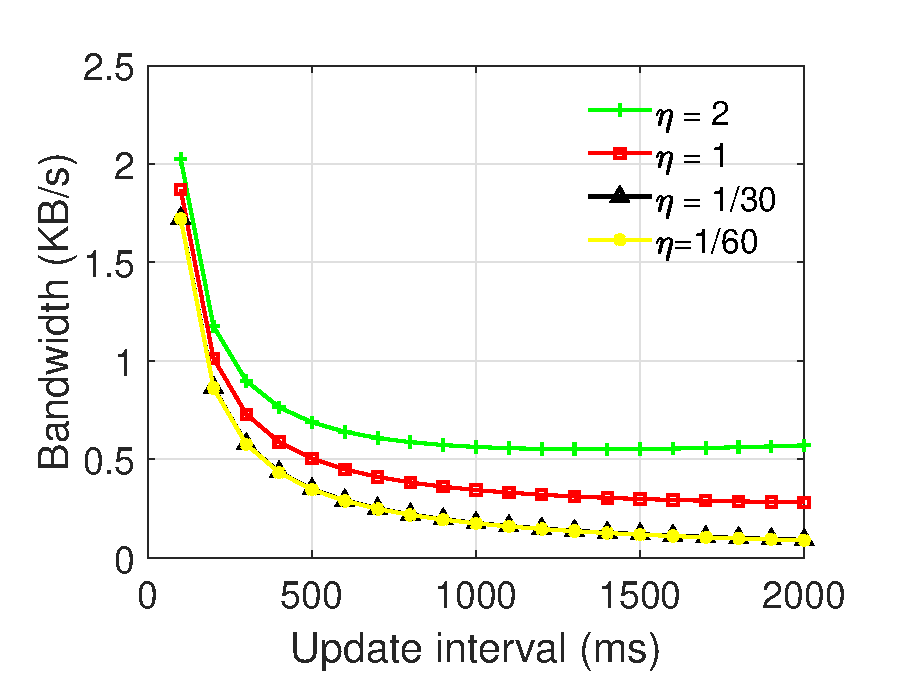
\includegraphics[width= 3 in]{expr/bandwidth}
    \caption{带宽开销}
    \label{fig:bandwidth}
  \end{minipage}
  \begin{minipage}[b]{0.49\textwidth}
    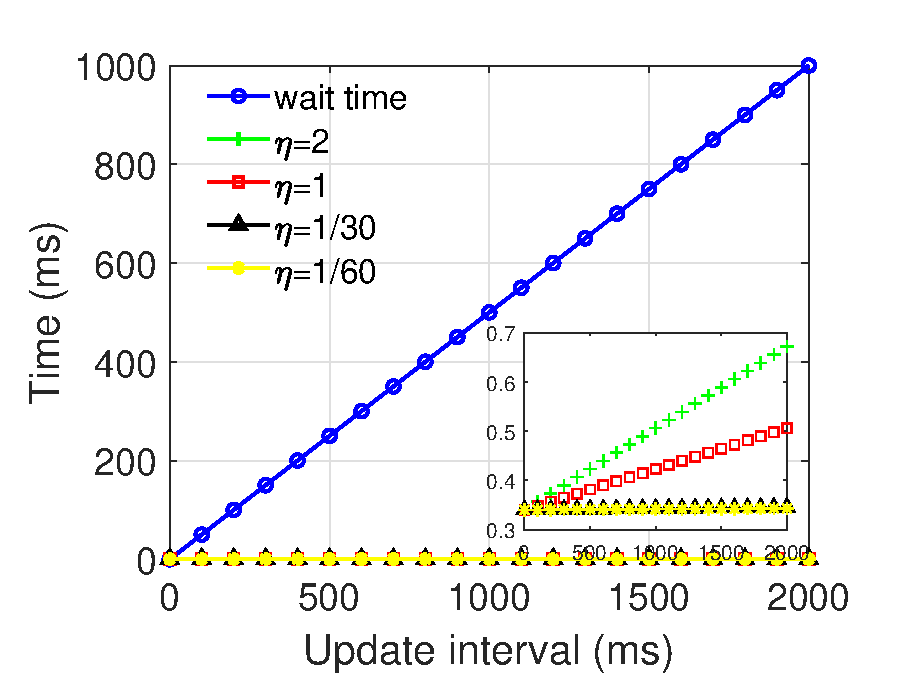
\includegraphics[width= 3 in]{expr/verify-2}
    \caption{总验证时间开销}
    \label{fig:verify-2}
  \end{minipage}
\centering
\end{figure}


In Fig.~\ref{fig:verify-2}, we evaluate the verification delays in data users. Note that an entire verification delay includes the delay of waiting for a checkpoint and the delay of executing the {\it Check} and the {\it Generate} algorithms. Since the execution delay of the {\it Generate} algorithm is relatively stable, around 0.1 milliseconds, we do not plot it in Fig.~\ref{fig:verify-2}. Here, $\eta$ is the update frequency of the data owner. We assume that the time that a user initiates a query is uniformly distributed during an update interval, and then the user's waiting delays are also uniformly distributed. Therefore, the expected delay is half of the update interval and the verification delays are dominated by the waiting delays. The execution delay of the {\it Check} algorithm is negligible and is proportional to the update interval, which is mainly incurred by verifying the signature and decrypting authenticators.
Kindly note that in above measurement, we do not take into account the network transmission and propagation delays, as they vary in different specific network contexts and do not reflect the essential extra cost directly introduced by our verification design. We do, however, report the communication overhead in terms of the message size, as shown in Fig.~\ref{fig:bandwidth}. In a later experiment, we will also show that we can set an update interval so as to make a trade-off between verification delays and communication overhead.

Fig.~\ref{fig:bandwidth} shows the bandwidth costs for authenticator update. %Here, $b$
Here, the size of the first authenticator in each update interval is around 112 bytes, which includes 32 bytes of the root of MPT, 8 bytes of the timestamp, an 8 bytes AES-CBC extension and a 128 bytes RSA signature. Overall, the bandwidth of the authenticator includes two part: the overhead introduced by the fixed update time point and the overhead introduced by data update. We can observe that the bandwidth cost increases to about 2KB per second when the update interval decrease to zero, this is introduced by the fixed update time point which is inversely proportional to the bandwidth overhead. Moreover, the bandwidth gradually increases when the update interval becomes too long. This overhead is introduced by the length of the authenticator, because as the update interval grows, the length of the authenticator becomes larger. Overall, the cost should be acceptable to achieve \multi. According to the results, in order to make a decent tradeoff between verification delays and bandwidth costs, we suggest choosing an update interval between 500 milliseconds and 1,500 milliseconds.

图9和图10评估了系统的总验证开销,包括计算开销和通信开销。我们主要考虑合法用户端的验证计算开销,和数据拥有者端的通信开销。图中的η表示数据拥有者的数据更新频率。
首先,我们考虑合法用户端的验证开销。这部分开销包括用户等待检测点的时间以及执行Check算法和Rebuild算法的时间。由于Rebuild算法的开销可以忽略,因此图9中并未标注该部分开销。如图9所示,蓝色的曲线表示合法用户等待检测点的时间,这里我们假设合法用户的查询时刻在一个更新周期内呈均匀分布,那么用户等待时间的均值就是更新间隔的一半。其余的曲线表示Check算法的执行时间,可以看到,当更新频率在2Hz到1/60Hz不等时,Check算法的执行时间也几乎可以忽略,因此合法用户端的验证开销主要取决于等待检测点所需的时间,即和更新间隔的设置有关。
其次,我们考虑数据拥有者端的通信开销。我们主要考虑由鉴别符带来的开销。由于鉴别符的更新包含两种情况,固定更新导致的鉴别符更新和数据更新导致的鉴别符更新。图10中的曲线充分体现了这两种更新带来的开销。首先,当数据拥有者的更新间隔设置的很小时,通信开销较大,这是因为固定更新太频繁导致的鉴别符的通信开销增大;当数据拥有者的更新间隔设置的很大时,通信开销也较大,这是因为当更新频率一定时,更新间隔越大,在更新间隔内形成的鉴别符的长度会累积增大,最终导致了鉴别符的通信开销增大。
综合以上两种情况,更新间隔可以设置为1000ms至1500ms之间。
